\chapter{Trabajo Desarrollado}
\label{chap:desarrollo}
\vspace{0.5cm}

%%%%%%%%%%%%%%%%%%%%%%%%%%%%%%%%%%%%%%%%%%%%%%%%%%%%%%%%%%%%%%%%%%%%%%%%%%%%%%%%
% Objetivo: Exponer las partes relevantes de la implementación                 %
%%%%%%%%%%%%%%%%%%%%%%%%%%%%%%%%%%%%%%%%%%%%%%%%%%%%%%%%%%%%%%%%%%%%%%%%%%%%%%%%

\section{Metodología}
\label{sec:metodology}
\lettrine{E}{s} difícil hablar de una planificación del proyecto como tal ya que por sus particularidades se han amalgamado características de varias metodologías. Lo que sí está claro es que el proyecto ha seguido una metodología ágil debido a su carácter de desarrollo evolutivo y orientado a la creación de prototipos funcionales en cada iteración. Se podría considerar que está a medio camino entre SCRUM y un ciclo de desarrollo en espiral con prototipado, ya que ha sido un proceso iterativo. Sin embargo, no es correcto decir que se ha utilizado SCRUM como metodología al no ser fácil repartir las tareas de cada iteración ni tener con quién hacerlo por ser un trabajo desarrollado por un único alumno junto con su director. 

La similaridad con el ciclo de desarrollo en espiral reside en que en cada iteración se pasan por los mismo puntos, revisando y modificando cada uno de los componentes para llegar al prototipo objetivo. Tras el trabajo, dicho prototipo es revisado en la reunión con el ``cliente'', que en este caso es el director del proyecto, revisando la funcionalidad implementada y dirigiendo los siguientes pasos.

Pese a las dificultades, disponiendo de una agenda de producto similar a la de SCRUM a modo de requisitos, se han podido trazar una serie de iteraciones. Cada iteración cuenta con su agenda de iteración en la cual se detallan los requisitos del prototipo a crear en ese paso haciendo evolucionar cada uno de los componentes. Se habla de hacer evolucionar los componentes y no de incrementarlos porque, pese a que cada iteración ha procurado incrementar la funcionalidad total del sistema, algunos módulos del mismo han sido refactorizados\footnote{Es decir, se ha cambiado su diseño, sin alterar su propósito funcional} en determinados pasos.

En cuanto a la planificación de pruebas del sistema, si bien se ha contado con diferentes entradas con las que probar cada uno de los módulos que se han ido desarrollando junto con el proyecto, no se puede decir que el desarrollo de una herramienta de estas características pueda ser dirigido por la prueba, ya que las soluciones halladas mediante \textit{Answer Set Programming} no pueden ser establecidas de antemano debido a su carácter no determinitsa.

Se estableció que la duración de cada iteración sería, en promedio, de semana y media. Esto equivale a unas 40 horas de trabajo por iteración, aunque se decidió permitir la flexibilización de las iteraciones ante imprevistos en el desarrollo. Esto no se corresponde con una metodología SCRUM típica en la que habría que desplazar tareas a las siguientes iteraciones, pero al ser solo una persona encargada de todo el trabajo, se decidió dotar a la metodología de cierta flexibilidad para no arrastrar trabajo. No obstante, esta flexibilización permite también ganar tiempo, ya que de completarse el trabajo antes de lo previsto se podría acortar el tiempo dedicado a alguna iteración.

Gracias a esta flexibilidad se logró depender solo de completar los objetivos de las diferentes agendas, logrando así independencia del factor tiempo, que ya venía fijado por los plazos de entrega propios del proyecto. 

\section{Planificación}
\label{sec:planning}
Debido a estos factores derivados de lo particular de desarrollar un sistema basado en \textit{Answer Set Programming}, se carece de una planificación inicial cerrada y completa que marque el tiempo estimado para cada una de las tareas en forma del tradicional diagrama de Gantt. No obstante, a modo de registro, sí se ofrece un diagrama similar que muestra el tiempo invertido en cada una de las iteraciones (Figura \ref{fig:tareas}).

\begin{figure}
	\centering
	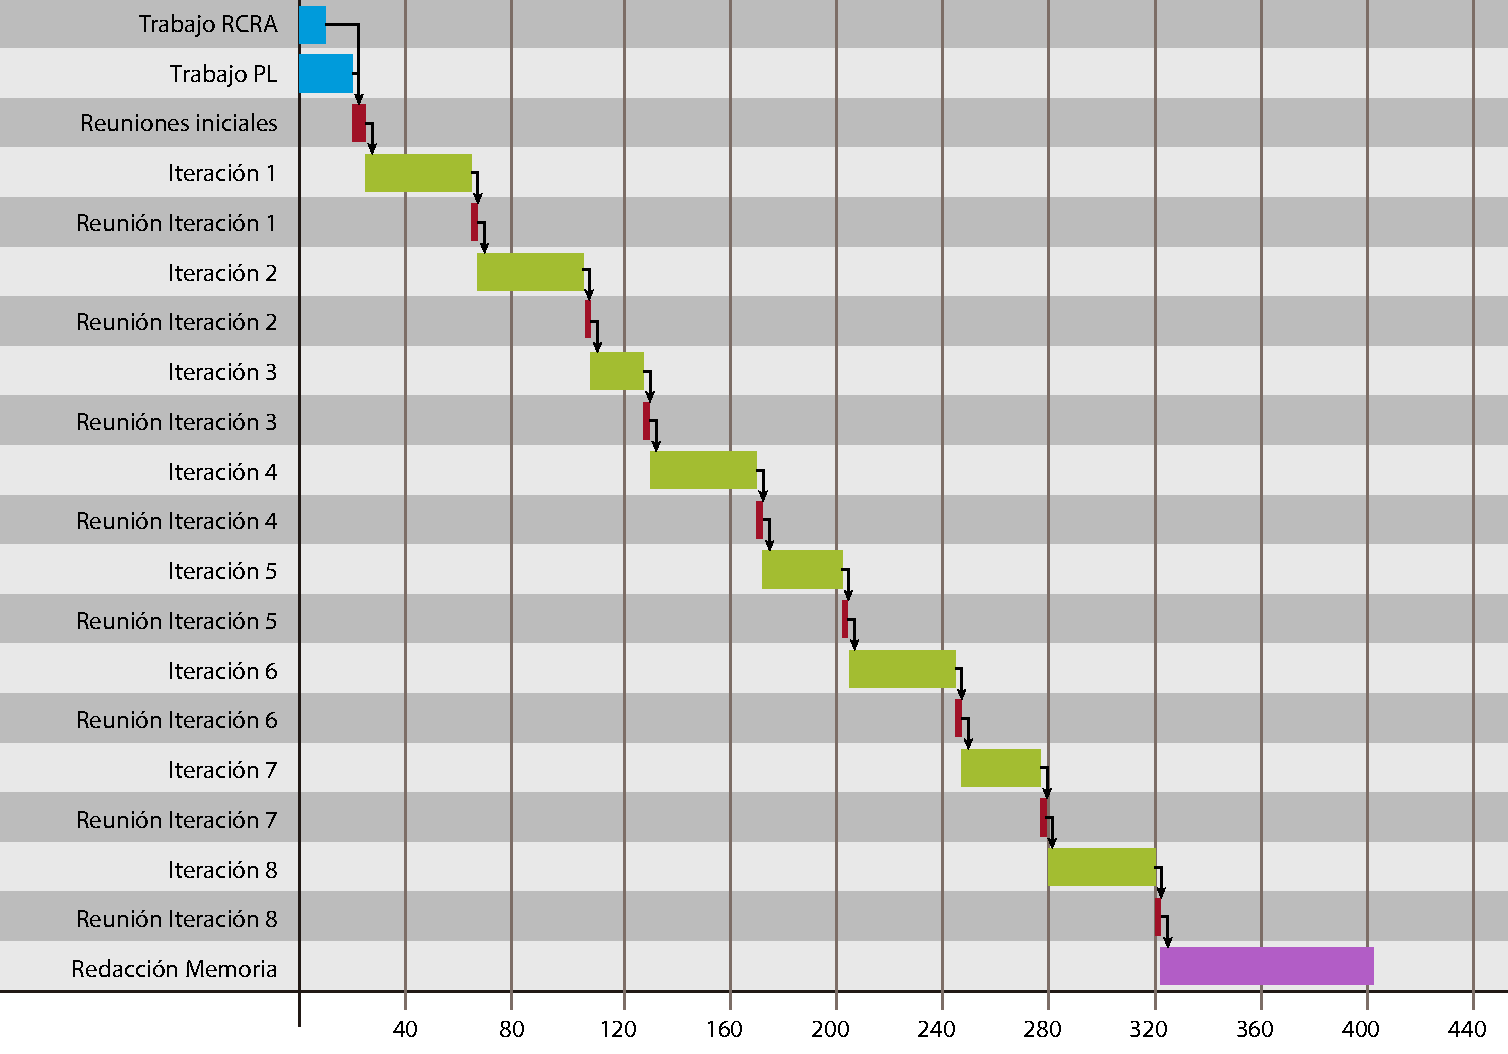
\includegraphics[width=0.8\linewidth]{imagenes/diagrama_tareas.pdf}
	\caption{Diagrama que muestra la secuencia de tareas}
	\label{fig:tareas}
\end{figure}

Dado este diagrama, es relativamente sencillo realizar una primera estimación del coste del proyecto. Hay que tener en cuenta, no obstante, horas extra de desarrollo que se incluyen en el diagrama y en el presupuesto ya que el trabajo no empezó de cero, al haberse realizado dos prácticas durante los años tres y cuatro del grado que se han reutilizado en menor o mayor medida para comenzar el desarrollo del presente trabajo. En la asignatura de ``Representación del Conocimiento y Razonamiento Automático'' se desarrolló una pequeña herramienta en \textit{Answer Programming} capaz de completar y componer pequeñas piezas musicales en forma de \textit{Canon}, mientras que en la asignatura de ``Procesamiento de Lenguajes'' se creó una primera versión del procesador de MusicXML a hechos lógicos. Se ha realizado una estimación de que, de no haber trabajado en la práctica de RCRA, se habrían necesitado unas 10 horas adicionales en los primeros pasos del desarrollo del módulo de armonización de este proyecto, mientras que de no haber realizado la práctica de PL se habrían necesitado unas 20 horas adicionales.

Sumado a 40 horas por iteración y contando con 8 iteraciones, arrojan un total de 350 horas de desarrollo. Las reuniones de final de iteración duraron una hora escasa cada una, pero al haber habido más de una por iteración y que las primeras reuniones fueron más extensas al tener que definir y planificar el proyecto se estima que el proyecto contó con unas 12 horas de reuniones para las que hay que sumar el coste por hora del tiempo del director.

Se ha asignado un coste aproximado de hora de trabajo del proyectando de 5.5\euro{}/hora y un coste también aproximado de 9\euro{}/hora para el director del proyecto. Con un cálculo rápido el coste del proyecto suma 1925\euro{} por las horas de desarrollo, 66\euro{} por las horas de reuniones por parte del alumno y 108\euro{} por las horas de reuniones por parte del director, haciendo un total de \textbf{2099\euro{}} para el diseño y desarrollo completo del mismo.

El coste de producción del proyecto es esencialmente el mismo que el de desarrollo, ya que las licencias de todo el software utilizado son gratuitas y no requiere ningún tipo de hardware adicional para funcionar. Incluso el editor de partituras que se recomienda utilizar junto con el programa (MuseScore2) es libre y de código abierto.

\section{Desarrollo}
\label{sec:development}
La arquitectura de haspie es un sencillo pipeline escrito en Python con un único camino que se ejecuta siempre que se llama a la herramienta, este pipeline se encarga de llamar a cada uno de los submódulos, enmascarando así el comportamiento interno de cada uno de ellos. Este pipeline además permite en su llamada a través de línea de comandos especificar diferentes opciones que se pasan después a cada submódulo de forma individual, estas opciones pueden verse en detalle en el anexo \ref{chap:usage}.

\begin{figure}[h]
	\centering
	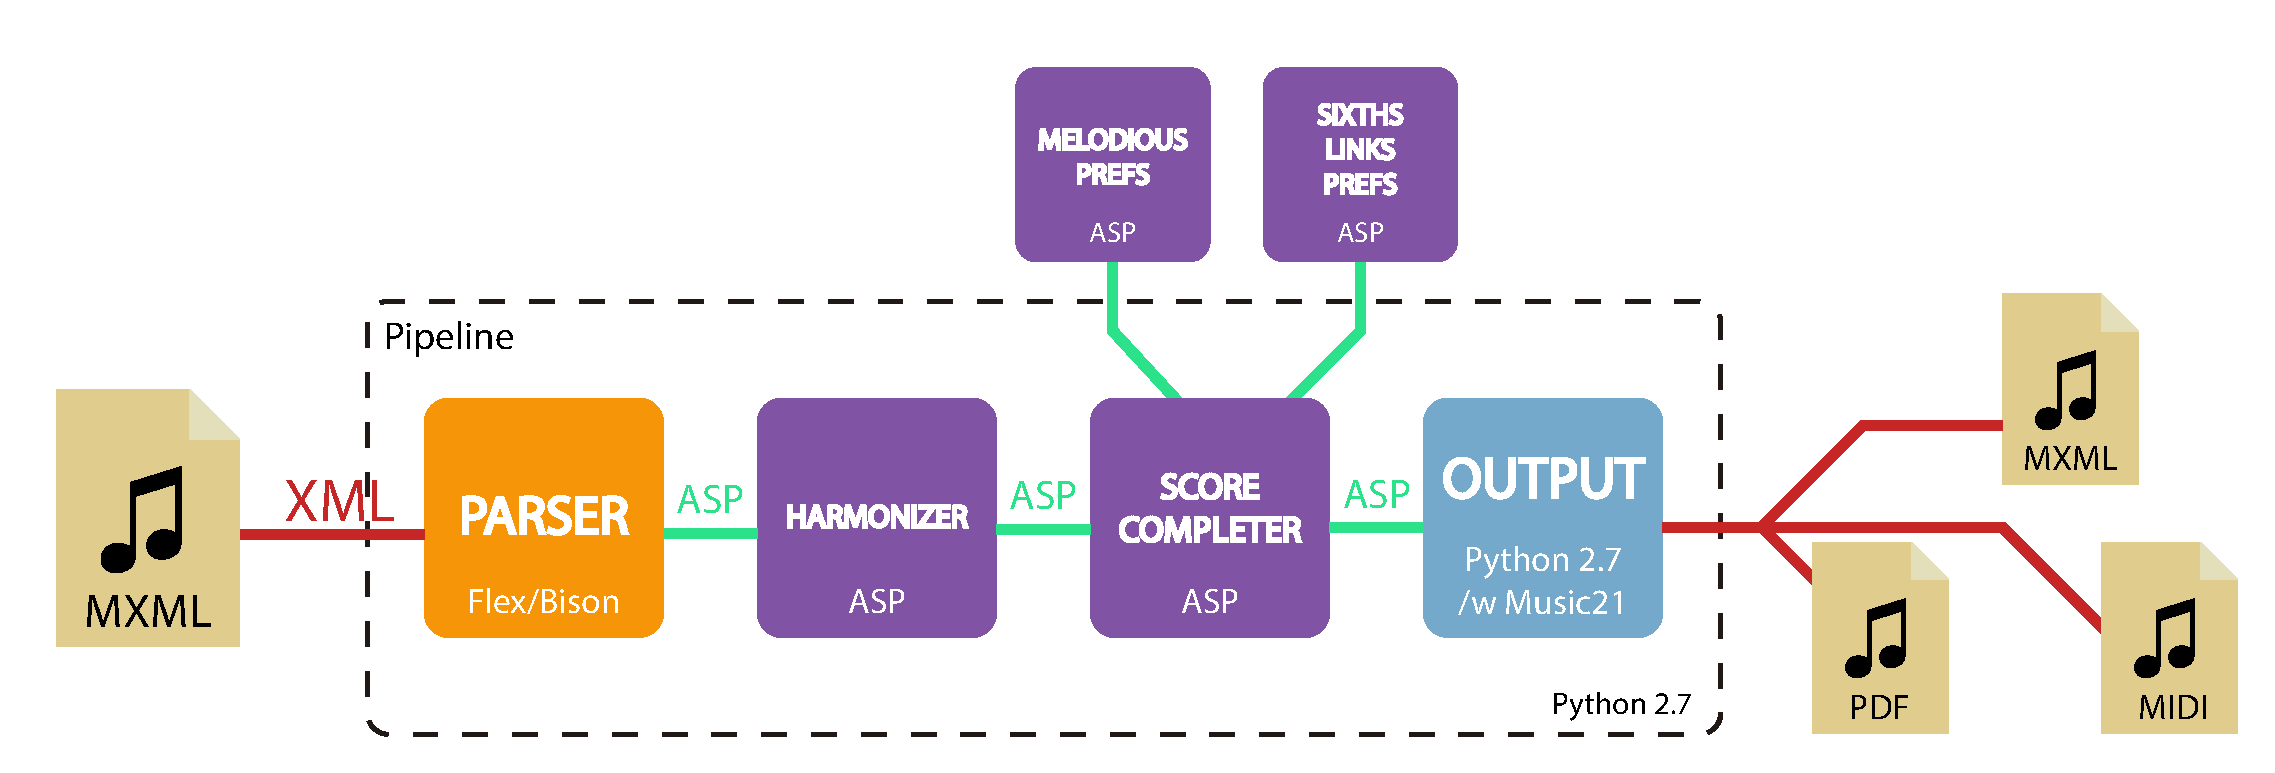
\includegraphics[width=0.8\linewidth]{imagenes/arquitectura_final.pdf}
	\caption{Arquitectura del sistema}
	\label{fig:arquitectura_final}
\end{figure}

\subsection{Entrada}
La entrada del sistema se realiza en formato MusicXML y el pipeline pasa la ruta del archivo especificado al módulo de entrada: un \textit{parser} escrito en C junto con las librerías Flex y Bison que se encarga de transformar los elementos de la partitura a hechos lógicos en Answer Set Programming. Este conversor no solo traduce las figuras y silencios a hechos sino que además:
\begin{itemize}
 	\item Subdivide todas las figuras de la partitura a la duración de la nota más breve de la pieza. Esta división es necesaria para que los módulos ASP puedan encajar correctamente todos los sonidos que se producen en cada tiempo de las diferentes voces de la pieza
 	\item Crea hechos lógicos adicionales \texttt{figure} que indican la duración original de cada una de las figuras con el fin de conservar esta información para que la pieza pueda ser reconstruida tras su procesado.
 	\item Itendifica las definiciones de la métrica de los compases que aparecen a lo largo de la partitura y convertirlos a los hechos lógicos correspondientes de modo que se pueda identificar correctamente el tipo de subdivisión de la partitura
 	\item Interpreta los nombres de los diferentes instrumentos de cada parte de la pieza y asigna hechos que vinculan cada una de las voces a un nombre instrumento o tipo de voz para poder detectar su tesitura
 	\item Lee la armadura de la partitura y determina la tonalidad y modo más probables correspondientes a la misma
 	\item Detecta el nombre y el autor de la partitura para poder representarlos en la salida
\end{itemize}
Aquellos datos procesados que no se convierten en hechos lógicos y se añaden al fichero ASP que servirá de entrada al núcleo dle programa se anotan en un fichero de configuración temporal que sirve a los distintos módulos del sistema para su funcionamiento.

El \textit{parser} funciona de un modo convencional, identificando las etiquetas relevantes que contienen la información necesaria para crear los hechos lógicos y almacenándolos en tipos de datos propio que se corrersponden con los elementos de la partitura tales como tipos de compás, anotaciones de acordes, nombres de instrumentos, nuevas voces, notas o silencios. A su vez, estos datos se almacenan en diferentes estructuras de cola (una para cada tipo de dato) mientras que se va procesando toda la pieza para calcular la longitud de la figura más breve. Una vez se ha terminado de leer la partitura, se extraen los datos de cada una de las colas y se procesan junto con la información general extraida al procesar toda la pieza para escribir los diferentes hechos lógicos en el fichero correspndiente o los metadatos y otros valores de salida en el fichero de configuración.

\begin{figure}[h]
	\centering
	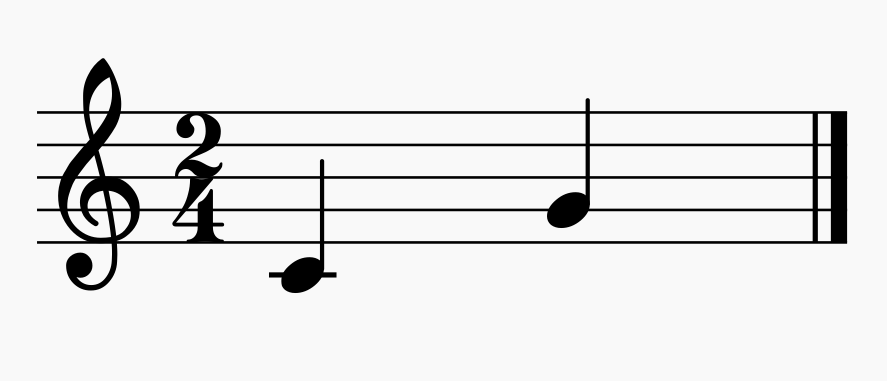
\includegraphics[width=0.4\linewidth]{imagenes/example_notes.png}
	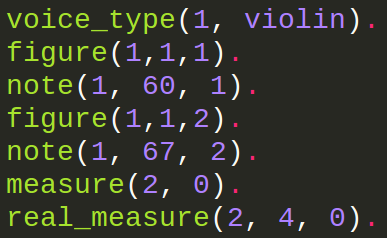
\includegraphics[width=0.4\linewidth]{imagenes/logic_facts_score.png}
	\caption{Una pieza simple transformada a hechos lógicos}
	\label{fig:simple-piece-facts}
\end{figure}

Además cuenta con parámetros en su llamada que modifican la salida producida:
\begin{itemize}
	\item \textbf{\texttt{-k}} Indica manualmente la clave en la que se armonizará la pieza en vez de detectarse automáticamente
	\item \textbf{\texttt{-s}} Especifica la cantidad de figuras consecutivas que se tienen en cuenta para la armonización
	\item \textbf{\texttt{-o}} Indica el nombre del fichero de hechos lógicos de salida	
\end{itemize}

\subsection{Núcleo ASP}
Los hechos lógicos creados por el \textit{parser} son la entrada directa del armonizador, una de las mitades del núcleo de procesado ASP de haspie.
Este módulo utiliza los hechos lógicos para expandir las reglas generales con las que cuenta, infiere nuevos predicados intermedios y asigna acordes de entre los posibles a cada tiempo de armonización especificado. Los posibles acordes se especifican en un archivo denominado \texttt{major\_chords} o \texttt{minor\_chords} según el modo en el que se esté realizando la armonización. Los acordes contemplados inicialmente por la herramienta son los acordes fundamentales de tres notas de la tonalidad, aunque se incluyó el de Dominante séptima\footnote{Acorde de cuatro notas que incorpora una nota adicional que forma un intervalo de séptima con la nota dominante de la tonalidad} para dotar al sistema de mayor naturalidad.

\begin{figure}
	\centering
	\begin{verbatim}
		1 { chord(HT,C) : pos_chord(C) } 1 :- htime(HT).
	\end{verbatim}
	\label{fig:chord-assig}
	\caption{Asignación de un único posible acorde a cada intervalo de armonización}
\end{figure}

\begin{figure}
	\centering
	\begin{verbatim}
		octave(V,((N - base) / 12),T) :- note(V,N,T), N >= 0.
		sem_tones(V,((N - base) \ 12),T) :- note(V,N,T), N >= 0.
		grade(V,1,T) :- sem_tones(V,3,T).
		grade(V,2,T) :- sem_tones(V,5,T).
		grade(V,3,T) :- sem_tones(V,7,T).
		grade(V,4,T) :- sem_tones(V,8,T).
		grade(V,5,T) :- sem_tones(V,10,T).
		grade(V,6,T) :- sem_tones(V,0,T).
		grade(V,7,T) :- sem_tones(V,2,T).
	\end{verbatim}
	\label{fig:grade-infer}
	\caption{Reglas de inferencia de Octava y Grado para una nota en el modo mayor.}
\end{figure}

Para ello, lo más importante es la conversión de los valores de las notas a grados de la escala junto con su octava, lo cual es posible conociendo la tonalidad y el modo. Con las notas transformadas en grados y todos los posibles acordes asignados, se cuantifican los errores cometidos, esto es, en vez de prohibir que se produzcan errores, se marcan aquellas notas que no pertenecen al acorde como error y se clasifican en errores fuertes y débiles atendiendo al tipo de tiempo del compás en el que coincide el error. El cálculo del tipo y subdivisión del compás, y por tanto de sus tiempos débiles y fuertes se realiza gracias a los hechos lógicos referentes al tipo de compás de la partitura y al intervalo de armonización de la misma.
Mediante un predicado de optimización que minimiza los errores en tiempos fuertes, los acordes repetidos en tiempos de armonización consecutivos y los errores cometidos en tiempos débiles (inicialmente en ese orden de importancia) se busca la mejor armonización posible.

\begin{figure}[h]
	\centering
	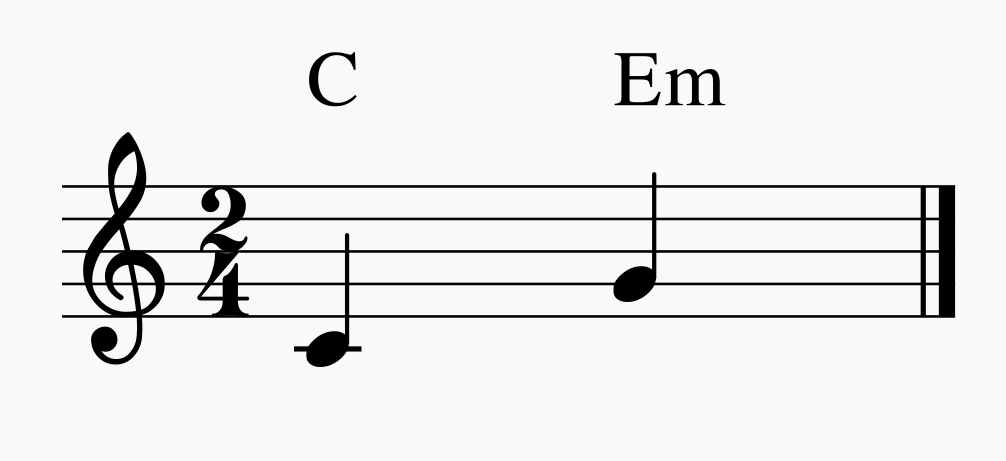
\includegraphics[width=0.4\linewidth]{imagenes/harmonized_example.png}
	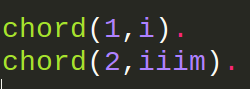
\includegraphics[width=0.4\linewidth]{imagenes/chord_facts.png}
	\caption{Acordes anotados sobre una pieza sencilla y los hechos lógicos correspondientes a esos acordes}
	\label{fig:simple-piece-chords}
\end{figure}

De vuelta al pipeline, los mejores resultados son transformados a una representación objetual en python (Ver sección \ref{subsec:store_classes}) para almacenar la información de los diferentes elementos y poder representarlos de manera sencilla. 

A continuación se pide al usuario que escoja un resultado de entre los mejores posibles, mostrándole la secuencia de acordes y especificando las notas erróneas, así como el grado de optimización del resultado. Una vez escogida la armonización deseada, se crea un fichero temporal con los acordes de la solución que se pasa, en conjunto con el fichero de hechos lógicos original al módulo de completado de partituras.

Con ambos ficheros de hechos lógicos, se llama al módulo de completado de partituras, que actuará en caso de existir voces nuevas que completar o secciones en blanco que rellenar. Los intervalos a rellenar están representados por el hecho lógico especial \texttt{freebeat} que indica que ese tiempo no contiene una nota sino un hueco intencialmente blanco. No obstante, estos hechos van acompañados de un hecho \texttt{figure} al igual que las notas o silencios, de modo que se puede especificar el patrón rítmico de la sección a completar.
El módulo de completado de partituras funciona de un modo similar al de acordes, asignando nuevas notas a los espacios en los cuales se le pida que lo haga. La principal diferencia es que no cuenta con un fichero de notas posibles como el módulo de armonización con los acordes, sino que utiliza el valor numérico de la nota directamente. 

\begin{figure}
	\centering
	\begin{verbatim}
		1 { freebeatfigure(V,N,1,FB) : N=VL..VH } 1 :- freebeat(V,FB),
		                 voice_limit_low(V,VL), voice_limit_high(V,VH).
	\end{verbatim}
	\label{fig:note-assig}
	\caption{Asignación de nuevas notas a espacios en blanco, respetando la tesitura especificada}
\end{figure}

Para limitar el espacio de búsqueda, estos valores son únicamente los comprendidos entre los límites definidos por la tesitura del instrumento de la voz que se esta está completando. De manera parecida al fichero de definición de los acordes de cada modo, se han definido las tesituras de algunas de las voces corales más frecuentes junto con algunos instrumentos como el violín o el violonchelo, así mismo este fichero puede ser fácilmente editado por el usuario para incluír nuevas tesituras o instrumentos.

\begin{figure}
	\centering
	\begin{tabular}{ | l | c | c | }
		\hline
		Tesitura & Nota mínima & Nota máxima \\ \hline \hline
		Bajo & 40 & 64 \\ \hline
		Barítono & 45 & 69 \\ \hline
		Tenor & 48 & 72 \\ \hline
		Contra-Tenor & 52 & 76 \\ \hline
		\hline
		Contralto & 53 & 77 \\ \hline
		Mezzo-Soprano & 57 & 81 \\ \hline
		Soprano & 60 & 84 \\ \hline
	\end{tabular}
	\label{fig:tesiturae}
	\caption{Relación de tesituras corales y sus límites inferior y superior}
\end{figure}

Estas nuevas notas se transforman a grados y octavas como ya se hace con las notas de entrada del módulo de armonización para poder ser cotejadas contra la armonía especificada por el módulo anterior. Del mismo modo que en el módulo de armonización se cuantifican y categorizan los errores porducidos por estas nuevas notas en relación a la armonía establecida y, minimizándolos, se buscan los mejores resultados. Gracias a los hechos lógicos \texttt{figure} de la entrada, el módulo de completado reconstruye las figuras originales.

\begin{figure}
	\centering
	\begin{verbatim}
		octave_jump(V,B1,B2) :- ex_note(V,N1,B1), ex_note(V,N2,B2),
		                     (B1+1) == B2, N2 > (N1+12), beat(B1+1).
		octave_jump(V,B1,B2) :- ex_note(V,N1,B1), ex_note(V,N2,B2),
		                     (B1+1) == B2, N2 < (N1-12), beat(B1+1).
		:- octave_jump(_,_,_).
	\end{verbatim}
	\label{fig:octave-jump}
	\caption{Definición de salto de octava para las notas generadas y restricción que lo prohibe}
\end{figure}

\begin{figure}[h]
	\centering
	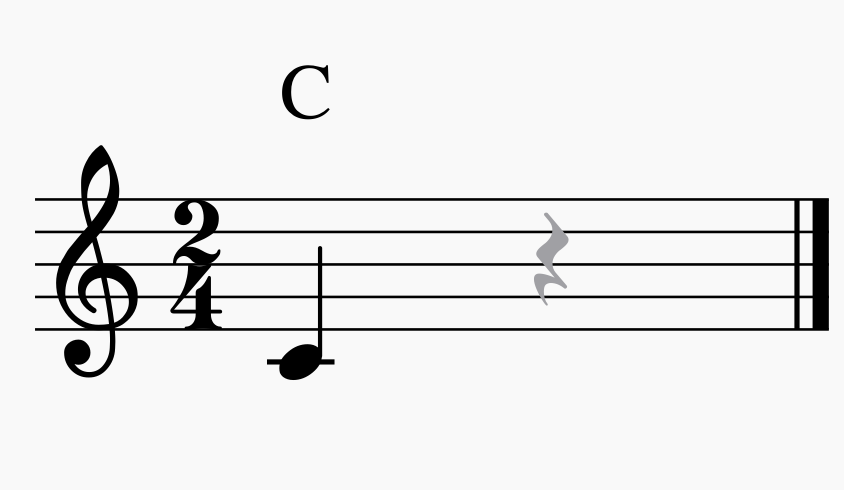
\includegraphics[width=0.4\linewidth]{imagenes/incomplete_score.png}
	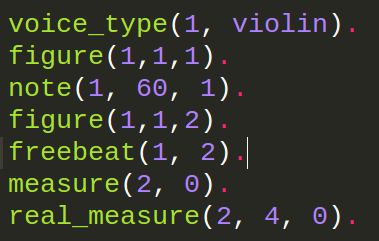
\includegraphics[width=0.4\linewidth]{imagenes/incomplete_facts.png}
	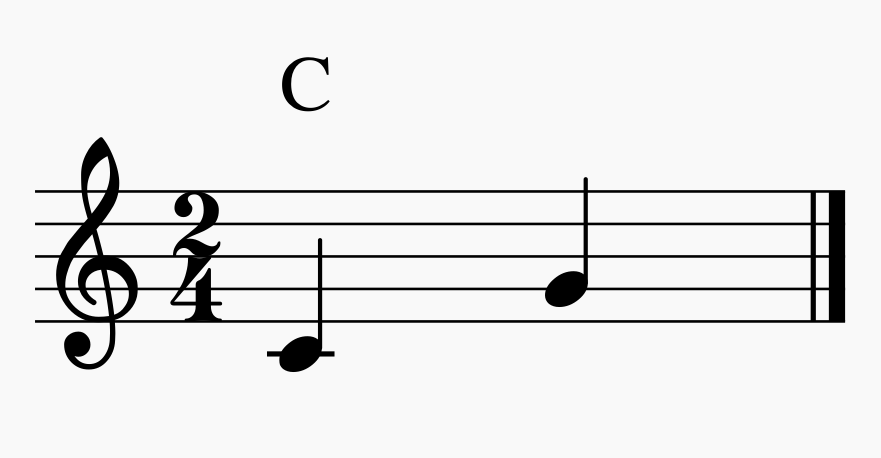
\includegraphics[width=0.6\linewidth]{imagenes/completed_score.png}
	\caption{Partitura armonizada con un tiempo incompleto y resultado del completado}
	\label{fig:simple-piece-complete}
\end{figure}

Repitiendo el proceso anterior, el pipeline procesa la salida de clasp y la almacena en las clases de almacenamiento correspondientes. Tras esto muestra las mejores soluciones de completado al usuario y permite escoger una de ellas. Al hacerlo los objetos de almacenamiento generados se pasan al módulo de salida para su representación final.

\subsection{Módulos de Preferencias}
Se han especificado, a mayores de los módulos principales ya descritos, dos submódulos adicionales que mejoran los resultados del módulo completador de partituras.

El primero es un módulo de preferncias melódicas. Sirve para compensar la ausencia de composición melódica en haspie creando partituras más cantables o melódicas. Contiene reglas que:
\begin{itemize}
	\item Definen la tendencia de una voz ya existente en la partitura y permiten al completador de partituras componer de forma que se imite dicha tendencia
	\item Miden los saltos melódicos entre las notas de una misma voz e intentan acortarlos haciendo que la progresión melódica sea más cantable.
\end{itemize}

Para la tendencia, se mide si en un intervalo determinado, el valor de notas consecutivas crece o decrece y mediante una regla que establece el tipo de tendencia (semejante u opuesta) al procesar multiples voces al mismo tiempo. Por otra parte, para los saltos melódicos se crean nuevos predicados \texttt{melodic\_jump} teniendo en cuenta la diferencia de los valores de notas consecutivas en una misma voz.

\begin{figure} [h]
	\centering
	\begin{verbatim}
		melodic_jump(V,J,B1,B2) :- out_note(V,N1,B1), out_note(V,N2,B2),
		                       (B1+1) == B2, beat(B1+1), J = #abs(N1-N2). 
	\end{verbatim}
	\label{fig:melodic-jump}
	\caption{Definición de salto melódico}
\end{figure}


El segundo módulo detecta progresiones de un determinado tipo de acordes (inversiones de cuarta y sexta). Este tipo de progresión es muy común en música coral, y por tanto, los resultados usando este módulo con piezas corales resultan mucho más realistas. Para esto se realiza una armonización a tiempo, es decir, se asigna un acorde a cada instante de la pieza y se intentan detectar estas progresiones concretas de acordes con el fin de crearlas o continuarlas si ya existen con la ayuda de las nuevas notas generadas. Es debido a esta armonización a tiempo que este módulo es tremendamente pesado computacionalmente.

\subsection{Ficheros de Configuración}
Las reglas de optimización, ya sean maximización o minimización, presentes en los módulos y submódulos ASP asignan un peso y un orden de relevancia a los predicados que se cuantifican de cara a la optimización. Este peso por defecto puede ser sobreescrito mediante ficheros de configuración. Cambiando el peso de cada hecho se altera como de importante es la aparición de cada uno de esos hechos, mientras que cambiando el orden de relavancia se determina como se realizará el proceso de optimización al completo.
Se presenta un fichero de configuración de ejemplo comentado para que el usuario pueda cambiar el funcionamiento de la herramienta a su antojo, produciendo cambios drásticos en el estilo con un esfuerzo mínimo y permitiendo almacenar estas preferencias en un fichero que determine su estilo personal de composición.

\subsection{Clases de Almacenamiento}
\label{subsec:store_classes}
Para poder almacenar temporalmente los resultados de los dos submódulos ASP de haspie se diseñaron e implementaron clases de almacenamiento que se corresponden con los diferentes hechos lógicos que los módulos ofrecen en su salida. El diagrama de clases de estos objetos de almacenamiento puede consultarse en el anexo \ref{chap:diagrams}. Se dividen en dos jerarquías, una para los resultados del módulo de armonización y otra, considerablemente más grande para el módulo de completado de partituras. 
En cuanto al módulo de armonización, éste cuenta con las siguiente clases:
\begin{itemize}
	\item \texttt{\textbf{ClaspChords:}} Almacena todas las solcuiones del armonizador, tanto en texto plano como en un array de objetos \texttt{ChordSolution}. Posee un método para transformar la salida de clasp a los diferentes objetos de la jerarquía.
	\item \texttt{\textbf{ChordSolution:}} Contiene dos listas ordenadas, una de objetos \texttt{Error} y otra de objetos \texttt{Chord}, y un valor de optimización que mide como de buena es la solución.
	\item \texttt{\textbf{Error:}} Representa una nota errónea en la partitura, especificando voz y tiempo para ubicarla en ella, así como el grado musical que produce el error.
	\item \texttt{\textbf{Chord:}} Representa un acorde en la pieza, especificando el nombre del mismo y el tiempo al que ha sido asignado.
\end{itemize}

Las clases para almacenar la información de la salida del módulo de completado de partituras siguen una estructura similar al de armonización, pero la jerarquía es algo más compleja al tener mucha más información que representar:
\begin{itemize}
	\item \texttt{\textbf{ClaspResult:}} Funciona de modo muy similar a \texttt{ClaspChords}. Almacena todas las solcuiones del completador de partituras, tanto en texto plano como en un array de objetos \texttt{HaspSolution}. Posee un método para transformar la salida de clasp a los diferentes objetos de la jerarquía. 
	\item \texttt{\textbf{HaspSolution:}} De forma parecida a \texttt{ChordSolution}, almacena los diferentes objetos de la solución. La principal diferencia radica en que hace uso de un diccionario de datos, siendo los índices cada una de las voces de la pieza y almacenando en la entrada de cada índice una lista ordenada de los diferentes objetos de la partitura.
	\item \texttt{\textbf{Error:}} Funciona igual que \texttt{Error} en la jerarquía de clases del módulo de armonización. Representa una nota errónea en la partitura, especificando voz y tiempo para ubicarla en ella, así como el grado musical que produce el error.
	\item \texttt{\textbf{PassingNote:}} Nota errónea que cumple unas características particulares, como su ubicación en un tiempo débil de la partitura. Especifica la voz y el tiempo en el que se produce, de modo similar a \texttt{Error}.
	\item \texttt{\textbf{Chord:}} Similar a \texttt{Chord} en la jerarquía de clases del módulo de armonización. Representa un acorde en la pieza, especificando el nombre del mismo y el tiempo al que ha sido asignado.
	\item \texttt{\textbf{VoiceType:}} Indica el nombre asignado a una voz, es decir, el instrumento que la interpreta.
	\item \texttt{\textbf{Note:}} Especifica la voz y tiempo en los que suena la nota, así como su valor numérico y duración.
	\item \texttt{\textbf{Rest:}} Especifica la voz y tiempo en los que se produce el silencio así como su duración.
	\item \texttt{\textbf{Measure:}} Indica la métrica del y cantidad de notas del tipo de compás así como el tiempo en el que aparece. Se interpreta que el cambio de tipo de compás se produce en todas las voces a la vez.
	\item \texttt{\textbf{VoiceChord:}} Representa un conjunto de notas que suenan en un mismo tiempo de una sola voz, produciendo un acorde (Por ejemplo en instrumentos polifónicos como el piano o la guitarra). Contiene un array de objetos \texttt{Note} ordenados por su valor numérico, así como la voz y el tiempo en el que se produce junto con su duración.
\end{itemize}


\subsection{Salida}
El último módulo al que llama al pipeline. Haciendo uso de los objetos de representación interna, el módulo de salida genera un fichero en el formato deseado por el usuario. 
Para la implementación de este módulo se ha hecho uso de la librería Music21\footnote{http://web.mit.edu/music21/} desarrollada por miembros del MIT. Se traduce la representación interna de la partitura que el pipeline pasa al módulo de salida a la representación propia de Music21 para después con una simple llamada, reproducir o almacenar el resultado.
En este proceso de conversión, no solo se traducen las notas, voces y anotaciones de compás al formato propio de Music21, sino que además se combinan algunos de ellos para enriquecer la salida.
\begin{itemize}
	\item Los acordes, especificados en forma de grado de la tonalidad, se traducen al nombre y tipo de acorde correspondiente para ser anotados en la partitura
	\item Los errores en tiempos fuertes se marcan en la partitura coloreando en rojo las notas que los contienen
	\item Los errores en tiempos débiles se marcan en azul en la partitura indicando que son notas de paso o adornos
\end{itemize}

\begin{figure}[h]
	\centering
	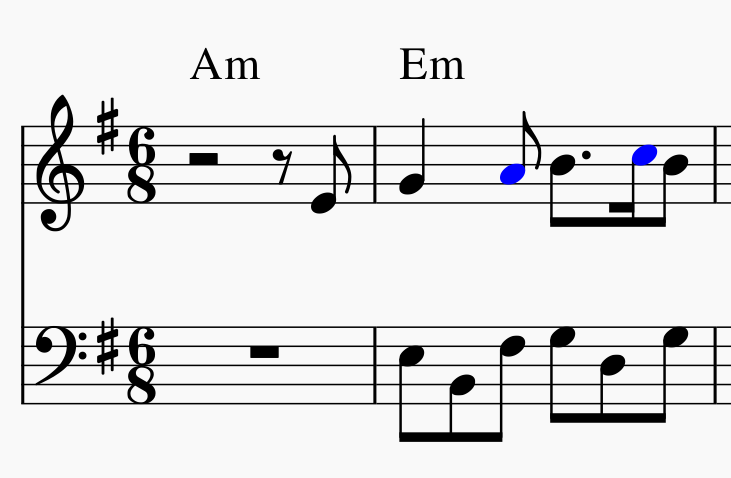
\includegraphics[width=0.6\linewidth]{imagenes/example_final_score.png}
	\caption{Partitura de ejemplo armonizada y con notas de paso coloreadas en azul}
	\label{fig:simple-piece-final}
\end{figure}


\section{Iteraciones}
Se detalla un breve resumen de cada una de las iteraciones de desarrollo del proyecto, indicando cuales fueron los progresos, cambios y refactorizaciones en cada una de ellas.

\subsection{Iteración 1}
\label{subsec:first_iteration}
Se analizaron y escogieron las diferentes tecnologías que se usarían en cada uno de los módulos de la herramienta. 
Como software de entrada para las partituras se escogió MuseScore 2, principalmente por ser \textit{opensource} y por su sencillez. Para el formato de entrada y salida, se compararon las propiedades de MIDI, LilyPond y MusicXML. Los tres formatos ofrecen posibilidades de edición, aunque cada uno sirve a un propósito diferente. MusicXML se presentó como el formato idóneo para la tarea, ya que al ser una extensión de XML, está orientado a que una máquina pueda procesarlo y crear una estructura en memoria con toda la información que necesita para poder extraer los datos de la partitura. Además, la implementación del \textit{parser} para un lenguaje etiquetado como XML es un problema convencional y relativamente sencillo.

Para el procesador de XML a hechos ASP se optó por las bibliotecas Flex y Bison para C. EL principal motivo para ello fue que fueron las tecnologías empleadas en la asignatura Procesamiento de Lenguajes y durante una de las prácticas de la misma se desarrolló una primera versión de este mismo procesador que ahora se usa en el proyecto. Además Flex y Bison garantizan velocidad y eficiencia en el procesado. Por último pero no menos importante, y ya que el proyecto se está enfocando desde un punto de vista de desarrollo ágil, actualizar los ficheros de código de Flex y Bison es realmente sencillo, lo cual permitiría añadir nuevos elementos a reconocer cuando sea necesario.

Se procedió a desarrollar una versión actualizada de dicho parser. Las pruebas realizadas al \textit{parser} revelaron que existía un problema de análisis al no poder verificar de forma sencilla que cada etiqueta se cerraba de modo correcto, es decir, que el nombre de la etiqueta que cierra un bloque sea el mismo del que la abrió, se implementó una pila en C para esta tarea. 

\begin{figure}
	\centering
	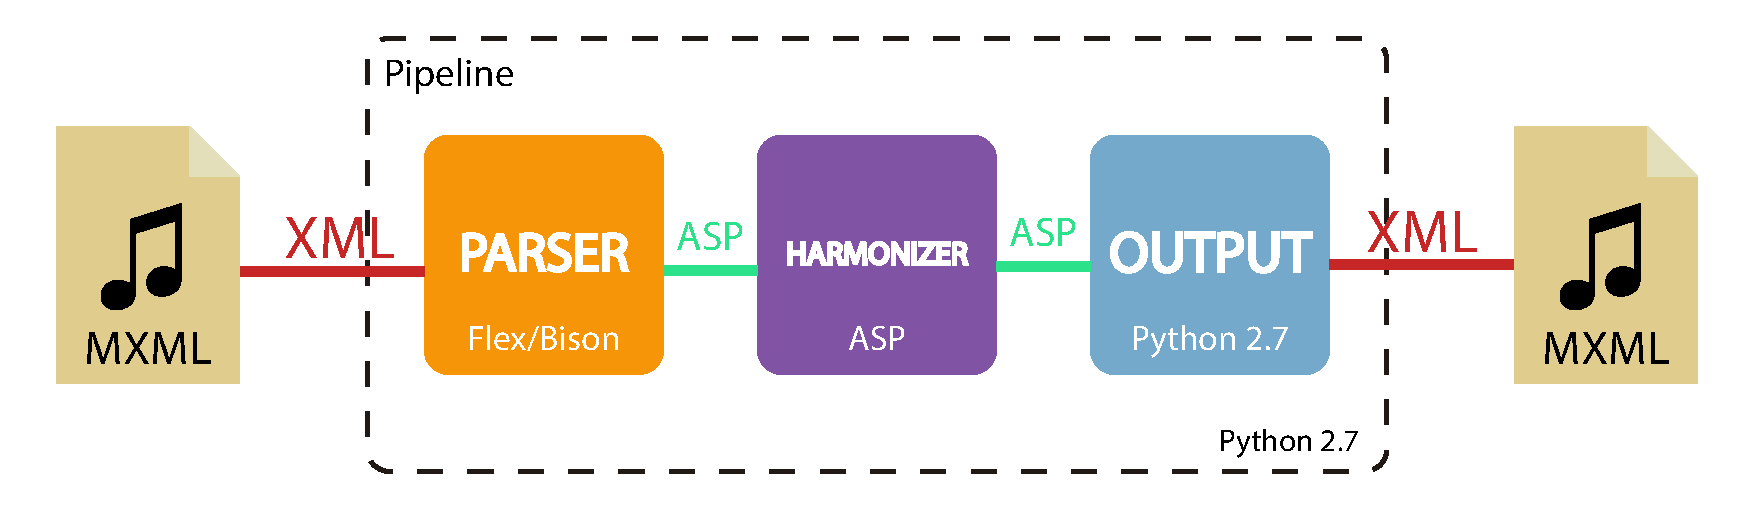
\includegraphics[width=0.8\linewidth]{imagenes/arquitectura_inicial.pdf}
	\caption{Diagrama del planteamiento inicial de la arquitectura del sistema}
	\label{fig:arquitectura_inicial}
\end{figure}

\subsection{Iteración 2}
\label{sec:second_iteration}
Se modificó el procesador de MXML a ASP y se incluyó una opción para subdividir la partitura de forma automática en base a la nota más breve de la partitura o forzar toda la partitura a un solo tipo de figura omitiendo aquellas figuras de menor duración.

En esta primera aproximación, se crearon las primeras reglas del módulo de armonización, que realizan una asignación acorde-unidad rítmica en base a las notas presentes para un instante dado en cada voz. Se crearon dos ficheros a mayores que especifican los acordes a considerar por la herramienta, según si la armonización se realiza en modo mayor o menor. 

A mayores se incluyó como parte de esta iteración, el diseño e implementación de un pipeline en python que automatiza las llamadas al procesador MXML a hechos ASP y al módulo de armonización. En este primer prototipo se implementó una pequeña funcionalidad de interpretación de la salida del módulo ASP a un vector de soluciones.


\subsection{Iteración 3}
\label{subsec:third_iteration}
Se modificó el \textit{parser} substancialmente ya que este imprimía a un fichero según procesaba las notas. Esto no planteaba problema alguno si la subdivisión se especificaba de antemano mediante el parámetro correspondiente, pero sí que resultaba complicado mantener esta aproximación si la unidad de subdivisión debía calcularse al mismo tiempo que se procesaba la partitura en MusicXML. Se plantearon dos soluciones: o bien incluir en el pipeline en python un análisis previo a la conversión de MXML a hechos en ASP que dedujese cual era la nota de menor longitud y la usase como parámetro en la llamada al \textit{parser} o bien se modificaba el comportamiento del anterior para realizar simultáneamente ambas tareas. 

Se optó por la segunda opción por motivos de coherencia con el sistema, es decir, no incluir funcionalidad innecesaria y replicada en el pipeline, cuya tarea es simplemente manejar las entradas y salidas de los diferentes módulos, y por motivos de eficiencia, ya que como se ha mencionado no hay necesidad de procesar el mismo fichero dos veces, siendo una de ellas en un lenguaje interpretado en vez de compilado, lo que añadiría un sobrecoste temporal evitable.

Los cambios implementados en el \textit{parser} conllevaron incluir un nuevo tipo de dato nota para almacenar la información de las notas de la partitura y una nueva pila que contuviese las notas extraídas del MXML.

En el módulo de armonización se incluyó una nueva constante que indica la longitud del intervalo de tiempo mínimo de análisis armónico horizontal. Se modificaron, por tanto, las reglas de asignación de acordes para poder usar el intervalo especificado. Además se suavizaron las restricciones que podaban las soluciones erróneas y en vez de ello, generan un nuevo predicado error(voz, grado, tiempo) que indica los grados erróneos presentes en la partitura que no encajan con el acorde asignado para la solución. 

 Se han implementado en el pipeline, con vistas al futuro de módulo de salida, una serie de clases para procesar y almacenar los resultados de clasp y poder devolverlos más tarde en el formato más conveniente. Concretamente, en esta iteración se implementaron las primeras versiones de \texttt{Error}, \texttt{Chord}, \texttt{HaspSolution} y \texttt{ClaspResult}.

\subsection{Iteración 4}
\label{sec:fourth_iteration}
El módulo ASP se ha aumentado para incluir generación de notas en un número de voces adicionales que puede ser especificado por parámetro. Además se refactorizaron algunas reglas y se creó un fichero de conversiones encargado de traducir valores de notas a grados, octavas y viceversa. Para la generación de notas en las nuevas voces se ha impuesto una única restricción fuerte: que dos notas consecutivas no realicen un salto melódico de más de una octava.

Se optó por incorporar \textbf{Music21} al módulo de salida. Principalmente por la cantidad de formatos con los que puede trabajar, tanto en entrada como en salida, y aunque lo ideal será exportar un fichero MusicXML, la idea de poder generar PDF, MIDI o Lilypond resulta más que atractiva. Este módulo toma un objeto \texttt{HaspSolution} y, previa transformación a la representación interna de Music21, lo representa en el formato adecuado para ser reproducido o almacenado.  

En el \textit{pipeline} se ha incluyó la opción de especificar el número de voces adicionales que deben ser añadidas y otra opción para especificar el formato de salida. A mayores, se incluyó una llamada al módulo de salida en el pipeline.

\subsection{Iteración 5}
\label{subsec:fifth_iteration}
En el procesador de MusicXML a hechos lógicos ASP se han incluido dos nuevas funciones principales: 
\begin{itemize}
	\item \textbf{Análisis de medida de compás:} Determinar cuantas figuras de qué longitud posee el tipo de compás base de la pieza.
	\item \textbf{Distincisón de tipos de silencios:} Diferenciar silencios completables de aquellos que deben ser respetados como silencios.
\end{itemize}

Para la métrica del compás, se implementó en el procesador la capacidad de identificar los diferentes tipos de compases así como el tiempo en el que ocurren, aunque por comodidad y sencillez, se ha asumido que un cambio rítmico en el compás debe ocurrir en todas las voces a la vez. El tipo de compás además es modificado según la nota mñas breve de la partitura para que no existan problemas a la hora de comparar la cantidad y el tipo de figuras del compás.

Para poder especificar en el editor de partituras silencios ``verdaderos'' y silencios completables se optó por una solución relativamente sencilla, no sólo de identificar por el \textit{parser} si no también fácil de usar por el usuario final de la herramienta. Mediante la notación de letras de la pieza, se pueden indicar en cada voz los intervalos de tiempo en los cuales los silencios deben ser tratados como completables. Para ello solo hace falta escribir los símbolos \texttt{[} y \texttt{]} al principio y final del intervalo respectivamente. Para poder detectar este intervalo se incorporó un tipo de dato cola genérica al procesador para poder interpretar bien el momento de inicio y de cierre de estos símbolos y marcar así los intervalos a completar de manera adecuada.

En el módulo de armonización se han definido acordemente varios predicados nuevos, que representan los tiempos completables de cada voz. A mayores de crearon reglas para identificar la subdivisión de los compases con el fin de inferir los tiempos fuertes y débiles de cada compás en la partitura. Gracias a esto se han creado predicados que matizan los diferentes errores de la partitura según el tipo de tiempo en el que ocurren los errores de la pieza y permite minimizarlos con diferentes prioridad (a más fortaleza de tiempo, más prioridad). Por último y para dar más flexibilidad en la búsqueda de la armonización correcta se ha incluído el acorde de dominante séptima (V7) en los modos mayor y menor.

Se ha incluido una clase de almacenamiento \texttt{Rest} para diferenciarla de \texttt{Note}. Ya que las entradas del diccionario que representa las diferentes voces de la partitura puede almacenar cualquier combinación de tipos de elementos, se estableció una convención para poder almacenarlos e iterar sobre ellos sin problema.

El módulo de salida se ha refinado para representar mejor las notas incluyendo información del tipo de compás, clave y duración de las figuras. Además se colorean en rojo los errores detectados y se anotan en los tiempos adecuados los acordes inferidos por el módulo ASP.

Por último, el pipeline cuenta con una nueva opción que permite especificar un tiempo máximo de búsqueda del óptimo en el módulo ASP, ya que para piezas largas, el espacio de búsqueda crece muchísimo y es necesario poder limitar el tiempo de ejecución.

\subsection{Iteración 6}
\label{sec:sixth_iteration}

Para facilitar la entrada de silencios que representan huecos completables por el módulo ASP se cambió el enfoque, y se abandonó el delimitado de secciones completables con corchetes en las letras de la canción por suponer algunos problemas al no poder ubicar dichas letras en tiempos en los que haya un silencio, por claridad y por no interferir con las posibles letras de una partitura real no creada ni modificada \textit{ad-hoc} para el programa. MusicXML permite marcar elementos de la partitura como no visibles, esto solo afecta a la hora de imprimir en papel dicha partitura y a nivel musical no interfiere con ningún elemento. Además, la visibilidad de una nota o silencio puede ser fácilmente alterada en cualquier editor de partituras desmarcando una casilla al clicar sobre dicho elemento, lo cual facilita mucho el marcado de estos tiempos completables. Esto se reflejó en el procesador de MusicXML a hechos lógicos, que en vez de contemplar los dos símbolos utilizados anteriormente, ahora solo tiene que comprobar la visibilidad de un elemento para determinar si asignar un tiempo completable a dicho tiempo.

Para refinar la subdivisión en tiempos débiles y fuertes, se reimplementaron tanto en el módulo ASP como en el procesador de hechos lógicos a MusicXML, esto fue debido a que no es sencillo establecer dichos tiempos aritméticamente sólo teniendo en cuenta la cantidad de notas del compás, sino que también se ha de tener en cuenta el tipo y subdivisión del compás con respecto a la nota de referencia usada para armonizar. Para esto es importante no normalizar el compás leído en el fichero XML y generar nuevos predicados indicando los valores del compás sin modificar. En el módulo ASP se ha incluido, de modo similar a los acordes, una tabla de tipos de compás y su subdivisión teniendo en cuenta el compás y la longitud del tiempo de armonización. Se han incluido en dicha tabla los compases más habituales. 

Se creó el sub-módulo ASP de preferencias melódicas que busca alcanzar una optimización mayor a la hora de generar nuevas voces o cubrir tiempos completables con algunas mejoras que atienden, principalmente, a la secuencia de notas de una misma voz. Se incluyó también en este sub-módulo de preferencias melódicas la detección de patrones de secuencias de sextas.

Se ha descartado la detección de apoyaturas con el fin de no contemplarlas como errores por un motivo similar, al uniformizar la longitud de las figuras de la partitura, no es posible detectarlas bien, ya que una de las características de las apoyaturas es que ``roban'' brevemente el tiempo fuerte a una nota representativa del acorde de la armonía.

\subsection{Iteración 7}
\label{subsec:seventh_iteration}

Se incluyeron en el \textit{parser} nuevos \textit{tokens} y reglas en la gramática para poder extraer metadatos y otra información de la partitura y exportarlos a un fichero temporal usado por el módulo de salida. Los diferentes datos extraídos para cada partitura son:
\begin{itemize}
	\item \textbf{title:} Título
	\item \textbf{composer:} Compositor
	\item \textbf{base\_note:} Longitud de la nota más breve presente
	\item \textbf{key\_name:} Nombre de la clave en la que se armonizará la pieza
	\item \textbf{mode:} Modo (mayor o menor)
	\item \textbf{last\_voice:} Número que identifica cual es la última voz presente
\end{itemize}

El procesador extrae una nueva pieza de información de la partitura, conocida como \texttt{figure}. Figure es un hecho lógico que describe la duración de una figura para un pulso de una voz dada. De este modo, pese a subdividir las notas a la longitud de la más breve para el análisis, se pueden recomponer en la salida fidedignamente. Se han incluido reglas adicionales para reconocer los acordes presentes en la partitura y estos se plasman en el fichero de salida.

En el módulo de armonización se ha incluido un nuevo archivo similar al de acordes o tipos de compases que describe las diferentes tesituras de las voces presentes en la partitura. Este documento es ampliable al igual que los mencionados para incluir nuevos instrumentos o tesituras. Se han definido los principales tipos de voz coral (tanto masculinos como femeninos) y sus rangos de notas más frecuentes. 

Además el módulo de armonización se añadieron reglas para tener en cuenta los nuevos hechos \texttt{figure} y utilizarlos para generar los patrones rítmicos adecuados en las secciones a completar. Para este mismo módulo se corrigió el archivo de preferencias de enlace de sextas, ahora separado del archivo de preferencias melódicas. Por último se ha adaptado la salida para trabjar con un nuevo hecho lógico que conjuga las notas con las figuras para producir un unico hechoconjunto con toda la información necesaria.

Se ha definido una nueva clase \texttt{VoiceChord}, que representa un acorde realizado por un solo instrumento polifónico ya que los este tipo de acordes producían fallos en la anterior iteración. Para su correcto funcionamiento se modificó la pequeña rutina de transformación de hechos lógicos de la salida del módulo de armonización para tener en cuenta la posibilidad de que existiesen varias notas en un mismo pulso de una voz y agregarlas en un objeto VoiceChord.

En el módulo de salida se han corregido algunos errores encontrados en las iteraciones anteriores y haciendo uso de los nuevos hechos lógicos de la iteración, se puede reconstruir la partitura mucho mejor que antes. Además el módulo de salida tiene en cuenta y representa correctamente el nuevo elemento \texttt{VoiceChord} y en la partitura además se escribe en la clave especificada o detectada por el procesador. Por último, se ha incluido una nueva funcionalidad para leer del archivo de temporal de configuracion de la partitura los metadatos de título y compositor, junto con los nombres de los instrumentos de cada pentagrama, que son asignados a cada una de las voces de la partitura de salida.

Los nuevos datos extraídos por el procesador son leídos desde el pipeline y son pasados a los subsiguientes módulos de armonización y salida respectivamente. Se ha modificado el parámetro -v del pipeline y su efecto en el resto de módulos. En vez de especificar una cantidad de voces a añadir, toma como mínimo un argumento indicando la tesitura (por nombre) o el rango de notas para las nuevas voces. El pipeline se encarga de crear, a partir de los datos de este parámetro -v un nuevo fichero temporal \texttt{extra\_voices.lp} que será incluido en la llamada del módulo de armonización para que dichas nuevas voces se tengan en cuenta. Se incluyó una opción que permite especificar manualmente la clave de la partitura mediante la letra de nota base de la escala en la que se quiere armonizar la pieza. De no ser especificada esta se calcula automáticamente. Cuenta además con otra opción que permite incluir la preferencia de los enlaces de sextas.

Tras probar el prototipo de esta iteración se llegó a la conclusión de que había dos factores ralentizando el proceso:
\begin{itemize}
	\item La armonización se realizaba junto con el completado de voces y espacios en blanco, con lo cual ASP debía generar todas las posibles combinaciones de notas para todas las posibles armonizaciones.
	\item La generación de notas se calculaba para cualquier rango y después se restringía para la tesitura correcta en vez de generar notas entre los límites de la tesitura. 
\end{itemize}

\subsection{Iteración 8}
\label{subsec:eighth_iteration}
Se tomó la decisión de dividir el módulo de armonización en dos sub-módulos ASP:
\begin{itemize}
	\item \textbf{Armonización:} Busca fijar una armonización ofreciendo al usuario diferentes soluciones ordenadas según unos valores de optimización.
	\item \textbf{Completado:} Su trabajo será, una vez establecida la armonización deseada, completar la partitura de modo similar a como se realizaba antes.
\end{itemize}

Se realizaron cambios menores en ambas partes para adecuarlas a sus nuevas tareas, se eliminaron muchos componentes de salida y ciertas reglas de generación de predicados ahora inútiles en la asignación de acordes y se revisó el módulo de generación de notas para eliminar todo aquello referente a la asignación de acordes. Además en el módulo de generación de notas se restringió la generación de las mismas a aquellas posibles dentro de la tesitura de la voz.

Se diferenciaron los hechos \texttt{freebeat}, generados por el procesador y por tanto con un \texttt{figure} relacionado, de los pulsos a rellenar de las voces nuevas. Estos \texttt{newvoicebeat} se utilizan para realizar la asignación de las nuevas figuras y notas, de modo que ya se cree la figura de salida desde el principio. 
	
Para posibilitar la configuración de pesos y orden de optimización en los diferentes módulos y archivos de preferencias se cambiaron los valores constantes de las reglas de optimización por nombres de valores especificados en cada uno de los ficheros para que sirvan de valores por defecto. Se investigó sobre el orden de precedencia de los valores asignados a constantes en ASP y se descubrió que no se puede redefinir valores constantes y que el primer valor que toma es el usado. Esto se aplica a ficheros de configuración y los parámetros pasados por línea de comandos. Teniendo esto en mente, se creó un fichero de configuración \texttt{sample.lp} en la nueva carpeta pref, destinada a almacenar los diferentes ficheros de configuración de preferencias. Si este fichero se incluye en la llamada a clingo antes que cualquier otro fichero, los valores definidos en él serán los que se usen en el proceso de armonización y completado. Si alguno de los valores se borra en este fichero, se usará el valor por defecto. Además para poder trabajar con los módulos de preferencias opcionales que también contienen pesos y orden de optimización, se modificó el orden en el que estos ficheros se incluyen en la llamada a clingo.

Debido a estos cambios se modificaron las clases de almacenamiento para reflejar los resultados de la armonización y el completado de forma separada. De modo paralelo a las clases de almacenamiento \texttt{ClaspResult} y \texttt{HaspSolution} se crearon \texttt{ClaspChords} y \texttt{ChordSolution}.

Se revisaron errores producidos en la interpretación de los valores de las notas alteradas. El error se debía a una mala identificación por parte del \textit{parser} de los valores que podía tomar la etiqueta \texttt{alteration}. Se revisó también este módulo para corregir otro error que afectaba a instrumentos de varios pentagramas, donde las diferentes partes se dvididían en diferentes voces pero no se asignaba el nombre del instrumento de forma correcta a otras voces que no fuesen la primera.

Durante las pruebas finales se detectó un tipo de silencio no reconocido correctamente, este silencio usaba el símbolo de un silencio de blanca pero ocupaba todo el compás siempre, fuese cual fuese su duración. Tal y como estaba diseñado el procesador, que identificaba el tipo de figura y la subdividía cuando fuese necesario, este tipo de figuras eran irreconocibles y se tuvo que implementar un caso especifico para estos silencios especiales. 

En el pipeline se incluyeron dos nuevas opciones. Una para establecer el número máximo de soluciones deseadas y otra que permite pasarle a los módulos de armonización y completado de partitura el fichero de configuración deseado. Se cambió ligeramente el comportamiento del pipeline al tener que realizar las llamadas a los dos nuevos sub-módulos ASP, parando tras hallar las mejores armonizaciones y ofreciendo al usuario seleccionar la deseada y pasando el resultado al sub-módulo de completado, donde la ejecución continúa de modo similar a los anteriores prototipos. Por último se modificó la opción que permite especificar el tiempo límite de búsqueda para ser solo usada en caso de querer buscar todos los óptimos en vez de quedarse con el primero encontrado.


